\documentclass[conference]{IEEEtran}
\IEEEoverridecommandlockouts
% The preceding line is only needed to identify funding in the first footnote. If that is unneeded, please comment it out.
\usepackage{cite}
\usepackage{amsmath,amssymb,amsfonts}
\usepackage{algorithmic}
\usepackage[dvipdfmx]{graphicx}
\usepackage[dvipdfmx]{color}
\usepackage{textcomp}
\usepackage{xcolor}
\usepackage{comment}

\def\BibTeX{{\rm B\kern-.05em{\sc i\kern-.025em b}\kern-.08em
    T\kern-.1667em\lower.7ex\hbox{E}\kern-.125emX}}
\begin{document}

\title{SuiteRec: Automatic Test Suite Recommendation System Using Code Clone Detection Tool\\
{\footnotesize \textsuperscript{*}Note: Sub-titles are not captured in Xplore and
should not be used}
\thanks{Identify applicable funding agency here. If none, delete this.}
}

\author{\IEEEauthorblockN{1\textsuperscript{st} Ryosuke Kurachi}
\IEEEauthorblockA{\textit{Information Science} \\
\textit{Nara Institute of Science and Technology}\\
Nara, Japan \\
kurachi.ryosuke.kp0@is.naist.jp}
\and
\IEEEauthorblockN{2\textsuperscript{nd} Eunjong Choi}
\IEEEauthorblockA{\textit{dept. name of organization (of Aff.)} \\
\textit{Kyoto Institute of Technology}\\
Kyoto, Japan \\
echoi@kit.ac.jp}
\and
\IEEEauthorblockN{3\textsuperscript{rd} Given Name Surname}
\IEEEauthorblockA{\textit{dept. name of organization (of Aff.)} \\
\textit{name of organization (of Aff.)}\\
City, Country \\
email address or ORCID}
\and
\IEEEauthorblockN{4\textsuperscript{th} Given Name Surname}
\IEEEauthorblockA{\textit{dept. name of organization (of Aff.)} \\
\textit{name of organization (of Aff.)}\\
City, Country \\
email address or ORCID}
\and
\IEEEauthorblockN{5\textsuperscript{th} Given Name Surname}
\IEEEauthorblockA{\textit{dept. name of organization (of Aff.)} \\
\textit{name of organization (of Aff.)}\\
City, Country \\
email address or ORCID}
\and
\IEEEauthorblockN{6\textsuperscript{th} Given Name Surname}
\IEEEauthorblockA{\textit{dept. name of organization (of Aff.)} \\
\textit{name of organization (of Aff.)}\\
City, Country \\
email address or ORCID}
}

\maketitle

\begin{abstract}
It is important to support software testing to ensure software quality. In previous studies, various automatic generation techniques have been proposed to reduce test creation costs. However, automatically generated tests are usually not based on the process and intention of creating the target code, and are therefore generally considered to be less readable. And it makes later maintenance activities difficult. This places a question mark over their practical value. In this research, we propose SuiteRec, a tool that recommends existing high quality test codes that exist on OSS to solve this problem. SuiteRec considers test reuse between clone pairs using similar code search technology. SuiteRec detects similar codes from the input code and recommends a test suite corresponding to the similar codes to the developer. Further, SuiteRec shows the developer a test smells that means a bad implementation of the test code. and the recommendation ranking is sorted so that a higher quality test suite can be recommended. In the evaluation of the proposed tool, the test code was created depending on whether the subject used SuiteRec or not, and the difference was compared. With various experiments, we show that (1) SuiteRec is effective to increase code coverage when creating test code for programs with many conditional branches, (2) Using SuiteRec takes a lot of time to create test code, (3) The test code created using SuiteRec has a high quality with a small number of detected test smells, (4) When using SuiteRec, developers feel that it is easy to create test code, and they can be confident in the created code.

\begin{comment}
ソフトウェアの品質確保の要と言えるソフトウェアテストを支援することは重要です.これまでに,テスト作成コストを削減するために様々な自動生成技術が提案されてきました.しかし,自動生成されたテストコードはテスト対象コードの作成経緯や意図に基づいて生成されていないという性質から後のメンテナンス活動を困難にさせる課題があり,これは自動生成技術の実用的な利用の価値に疑問を提示させます.本研究では,この課題を解決するために,OSSに上に存在する既存の品質の高いテストコード推薦するツールSuiteRecを紹介します.SuiteRecは,類似コード検索ツールを用いてクローンペア間でのテスト再利用を考えます.入力コードに対して類似コードを検出し,その類似コードに対応するテストスイートを開発者に推薦します.さらに,テストコードの良くない実装を表すメトリクスであるテストスメルを開発者に提示し,より品質の高いテストスイートを推薦できるように推薦順位がランキングされています.提案ツールの評価では,被験者によってSuiteRecの使用した場合とそうでない場合でテストコードの作成してもらい,テスト作成をどの程度支援できるかを定量的および定性的に評価しました.その結果,(1) 条件分岐が多いプログラムのテストコードを作成する際にコードカバレッジの向上に効果的であること,(2) SuiteRecを使用した場合,テストコードの作成に時間がかかること,(3) SuiteRecを使用して作成したテストコードは検出されたテストスメルの数が少なく品質が高いこと,(4) SuiteRecを使用してテストコードを作成した場合は使用しなかった場合と比べて開発者は,自身で作成したテストコードに自信が持てることが分かった.
\end{comment}
%This document is a model and instructions for \LaTeX.
%This and the IEEEtran.cls file define the components of your paper [title, text, heads, etc.]. *CRITICAL: Do Not Use Symbols, Special Characters, Footnotes, 
%or Math in Paper Title or Abstract.
\end{abstract}

\begin{IEEEkeywords}
 clone detection, recommendation system, software testing, unit test 
\end{IEEEkeywords}

\section{Introduction}
近年,ソフトウェアに求められる要件が高度化・多様化する一方,ユーザからはソフトウェアの品質確保やコスト削減に対する要求も増加している[1].その中でも開発全体のコストに占める割合が大きく,品質確保の要ともいえるソフトウェアテストを支援する技術への関心が高まっている.しかし,現状では単体テスト作成作業の大部分が人手で行われており,多くのテストを作成しようとするとそれに比例してコストも増加してしまう.このような背景から,ソフトウェアの品質を確保しつつコスト削減を達成するために,様々な自動化技術が提案されている.

既存研究で提案されているEvoSuite[2]は,単体テスト自動生成における最先端のツールである.EvoSuiteは,対象コードを静的解析しプログラムを記号値で表現する.そして,対象コードの制御パスを通るような条件を集め,条件を満たす具体値を生成する.単体テストを自動生成することで,開発者は手作業での作成時間が自動生成によって節約することができ,またコードカバレッジを向上することができる.しかし,既存ツールによって自動生成されるテストコードは対象のコードの作成経緯や意図に基づいて生成されていないという性質から可読性が低く開発者に信用されていないことや後の保守作業を困難にするという課題がある[3].このことは、自動生成ツールの実用的な利用の価値に疑問を提示させる.テストが失敗するたびに,開発者はテスト対象のプログラム内での不具合を原因を特定するまたは,テスト自体を更新する必要があるかどうかを判断する必要がある.自動生成されたテストは,自動生成によって得られる時間の節約よりも読みづらく,保守作業に助けになるというよりかむしろ邪魔するという結果が報告されている.

本研究では,この課題を解決するためにOSSに存在する既存の品質の高いテストコード推薦するツールSuiteRecを紹介します.SuiteRecは類似コード検出ツールを用いてクローンペア間でのテスト再利用を考えます.入力コードに対して類似コードを検出し,その類似コードに対応するテストスイートを開発者に推薦します.さらに,テストコードの良くない実装を表すメトリクスであるテストスメルを開発者に提示し,より品質の高いテストスイートを推薦できるように推薦順位がランキングされています.

提案ツールの評価では,被験者によってSuiteRecの使用した場合とそうでない場合でテストコードの作成してもらい,テスト作成をどの程度支援できるかを定量的および定性的に評価した.その結果,提案ツールの利用は分岐が多く複雑なプログラムのテストスイートを作成する際に,コードカバレッジを向上させることができることや,ツールを使用して作成テストコードの品質が高いことが分かった.また,定性的な評価として実験後にアンケートを実施し,推薦ツールを使った場合多くの被験者は自分の作成したテストコードに自信が持てることが分かった.


\section{BACKGROUND AND RELETED WORK}
\textbf{Unit testing.}単体テストの実行タスクでは,ソフトウェアを動作させ,それぞれのテストケースにおいてソフトウェアが期待通りの振る舞いをするかを確認する.テスト工程のコスト削減のため,テスト実行タスクにおいて,単体テストではJUnitなどのテスト自動実行ツールの利用が産業界で進んでいる.しかし,テスト設計タスクは未だ手動で行うことが多く,自動化技術の実用化および普及が期待されている.

単体テスト設計タスクで作成されるテストケースは,テスト手順,テスト入力値,テスト期待結果から構成される.テスト手順に従ってテスト対象のソフトウェアにテスト入力値を与え,その出力結果をテスト期待結果と比較する.これが一致していればテストは合格となり,一致しなければ不合格となる.単体テスト設計タスクにおいては,多くの場合同値分割法,境界地分析法などのテストケース作成技法を用いてテスト入力値を作成するが,ソフトウェアの要求通りに動作するかを確認するために多くのバリエーションのテスト入力値を作成する必要がある.

\textbf{Test case generation.}既存の研究[4]は,既存のテストケースを再利用,自動生成,または再適用できることによって,ソフトウェア開発のテスト工程における時間とコストを大幅に節約できることを示している.テスト生成技術は,主にランダムテスト(RT),記号実行(SE),サーチベーステスト(SBST),モデルベース(MBT),組み合わせテストの5つに分類できる.SEはさらに静的記号実行(SSE)と動的記号実行(DSE)に分けられる.

RTとは,ソフトウェアにランダムな入力を与えるテスト手法である.無造作・均一にテストを実行するランダムテストは自動化に適しているが,コードカバレッジ率向上,バグ検出の観点において,テストケース1件当たりの効率は著しく悪い.

SEは対象コードを静的解析してプログラムを記号値で表現し,コード上のそれぞれのパスに対応する条件を抽出し,パスごとにパスを通るような入力値が満たすべき条件を集める.そして,パスごとにその条件をSMTソルバ[5]などの制約ソルバを用いて解き,得られた具体値をテスト入力値とする.

SBSTは,達成したい要件に対する達成度合いを定量的に評価できるように設計した評価関数に基づいて,ヒューリスティック探索アルゴリズムを用いて達成したい要件を満足するテストスイートを生成する技術の総称である.

MBTはモデルに基づいてテストスイートを生成する技術の総称である.モデルは何らかの形でテスト対象を記述したものであり,要求分析や設計のためのモデルを活用することもあれば,テストのためにモデルを作成することもある.

CTは,パラメータ間の相互作用に起因する不具合を効果的に発見するためにテストケースとしてパラメータに割り当てる値の組み合わせを生成する手法である.

%\textbf{Test reuse using clone pairs.}

\textbf{Test Smell.}
プロダクションコードだけでなく,テストコードのも適切なプログラミングの慣習に従って設計する必要があります[44].テストコードのを適切に設計することの重要性は元々Beck[7]によって提唱されました.さらに,Van Deursenら[50]は11種類のテストスメルのカタログ,すなわちテストコードの良くない設計を表す実装とそれらを除去するためのリファクタリング技術を定義しました.このカタログはそれ以降,18個の新しいテスト臭を定義したMeszaros [42]によってより拡張されました。最近の研究では,テストスメルの存在は開発者のテストスイートの理解に悪い影響を与えるだけでなく,テストコードがプロダクションコード内の不具合を見つけるのにあまり効果的でなくなると言われています.

\section{SuiteRec}
SuiteRec takes a code fragment of a function unit from a developer as input code and searches for similar codes of the input code. Then, test suites corresponding to similar codes are sorted and presented to developers in order of priority.

Figure 1 shows the flow until a test suite is recommended by SuiteRec. The recommendation method mainly consists of the following 4 steps.

\begin{comment}
SuiteRecは,開発者からの関数単位のコード片を入力とし,その入力コードの類似コードを検索します.そして類似コードに対応するテストスイートを優先順位の高い順に並び替え開発者に提示します.図1は,SuiteRecによってテストスイートが推薦されるまでの流れを示しています.推薦手法は,主に以下の4つのステップから構成されます.
\end{comment}

\begin{figure}[htbp]
\centerline{\includegraphics[width=8.5cm]{SuiteRec-outline.pdf}}
\caption{Overview of SuiteRec.}
\label{fig}
\end{figure}

\begin{enumerate}
\renewcommand{\labelenumi}{(\arabic{enumi})}
\item When SuiteRec receives a input code, it searches the source code repository for the corresponding similar code fragments using a existing code clone detection tool.
\item Detected similar code fragments, SuiteRec searches the test code repository for the test suite corresponding to the similar code.
\item SuiteRec detects test smells in the test suite collected by the previous step using existing test sumel detection tools.
\item As the final step, SuiteRec sorts test suites in descending order of priority based on similarity and number of test smells.
\end{enumerate}


\subsection{Code Clone Detection}
In this study, NICAD [3] was adopted as a similar code detection tool. NICAD converts code fragment layouts uniformly and detects code pairs by comparing code fragments in units of functions. By adopting such a method, NICAD has realized clone pair detection with high accuracy and high recall. NICAD searches the Github repository hosting large open source projects for similar code corresponding to the input code.

The source code repository in Fig. 1 contains only the production code of the Github project with test code. Specifically, we selected a project that had a test folder in the project and adopted the JUnit testing framework. NICAD has a project size limit that can be searched at once.  In order to shorten the search time, large-scale projects were divided, small-scale projects were integrated, and multiple search processes were run in parallel, making it possible to search for similar codes in real time. The detection setting is implemented in the proposed tool as a standard setting of NICAD.

\subsection{Test Code Detection}
In order to search for test suites corresponding to similar code fragments, the target code is associated with the test code. In this research, the following two steps are taken in order to precisely associate the test code with the target code.

\begin{figure}[htbp]
\centerline{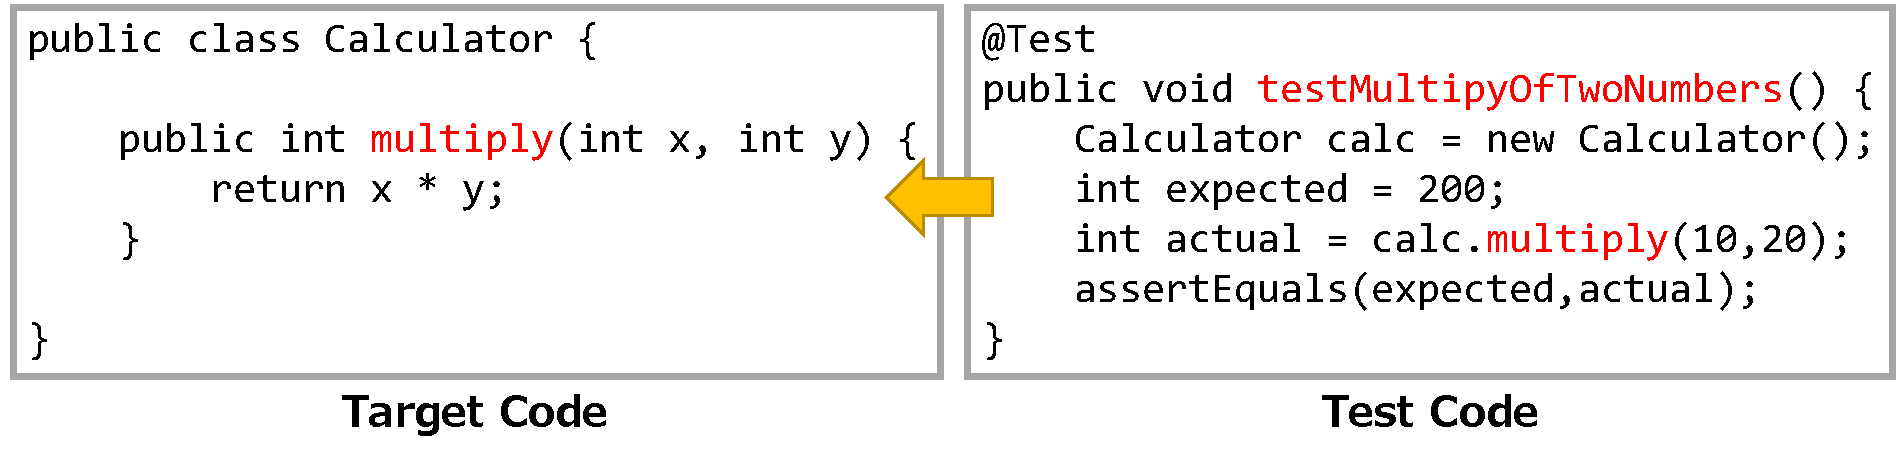
\includegraphics[width=8.5cm]{mapping.pdf}}
\caption{Example of mapping test code to target code.}
\label{fig}
\end{figure}

\begin{enumerate}
\renewcommand{\labelenumi}{(\arabic{enumi})}
\item Static analysis of test code and confirmation of method calls.
\item Divide the test method with a delimiter or capital letter and associate it when the target method partially matches.
\end{enumerate}


In the unit test, an object is generated in the test code as shown in the figure 2, and it is executed by calling a method of the test target code. Therefore, the test code in the test code repository is statically analyzed and the method call is obtained to associate the test target code with the test code. However, multiple methods may be called in the test method, so the method names are also compared. It is recommended to faithfully represent the contents of the processing of the target method as the test method name description method, and the name of the target method is often described in the test method name. Therefore, the name of the test method is divided by a delimiter or capital letter, and it is linked if it partially matches the target method.

The test code repository in Figure 1 stores test code corresponding to the production code in the source code repository. As a pre-processing, static analysis was performed on a large-scale project in advance, and information that linked production code and test code was stored in the DB, so that test code could be searched at high speed via the DB.

\subsection{Test Smells Detection}
In this study, tsDetect [6] was adopted as a test sumle detection tool. tsDetect is a tool implemented with an AST-based detection method that can detect 19 test smells. It has also been reported that test smells can be detected correctly with 85\% to 100\% accuracy and 90\% to 100\% recall. In this study, we implemented the following 6 types of test smells, which are important in considering the recommendation of test codes among 19 test smells that can be detected by tsDetect.
\begin{table}[hbtp]
\caption{Subject Test Smells}
\begin{tabular}{|l|p{5.2cm}|}
\hline
\textbf{Name}                   & \textbf{Description}                                                                                                       \\ \hline
\textbf{Assetion Roulette}        & Occurs when a test method has multiple non-documented assertions. Multiple assertion statements in a test method without a descriptive message impacts readability/understandability/maintainability as it’s not possible to understand the reason for the failure of the test.  \\ \hline
\textbf{Conditional Test Logic} & Test methods need to be simple and execute all statements in the production method. Conditions within the test method will alter the behavior of the test and its expected output, and would lead to situations where the test fails to detect defects in the production method since test statements were not executed as a condition was not met. Furthermore, conditional code within a test method negatively impacts the ease of comprehension by developers. \\ \hline
\textbf{Default Test}            & Test code in which the test class or test method name is the default in test code using a testing framework such as JUnit. It is necessary to change the name appropriately to improve the readability of the code.                                                                                                      \\ \hline
\textbf{Eager Test }             & Occurs when a test method invokes several methods of the production object. This smell results in difficulties in test comprehension and maintenance. \\ \hline
\textbf{Exception Handling}      & This smell occurs when a test method explicitly a passing or failing of a test method is dependent on the production method throwing an exception. Developers should utilize JUnit's exception handling to automatically pass/fail the test instead of writing custom exception handling code or throwing an exception. \\ \hline
\textbf{Mystery Guest}          & Occurs when a test method utilizes external resources (e.g. files, database, etc.). Use of external resources in test methods will result in stability and performance issues. Developers should use mock objects in place of external resources. \\ \hline
\end{tabular}
\end{table}

In addition, the test code including the following four test smells that are not suitable as recommended test code has been deleted from the test code repository in advance, so that it is not output as a recommended test code. 

\begin{itemize}
\item \textbf{Empty Test.}Occurs when a test method does not contain executable statements.
\item \textbf{Ignored Test.}Test code that has the @Ignore annotation and is not executed.
\item \textbf{Redundant Assertion.}This smell occurs when test methods contain assertion statements that are either always true or always false. 
\item \textbf{Unknow Test.}A test method that does not contain a single assertion statement and @Test(expected) annotation parameter.
\end{itemize}

\subsection{Sort Recommended Test Suites}
The recommended test suites were ranked based on the similarity between the input code and the detected similar code and the number of test smells included in test suites. We investigated the relationship between the similarity between clone pairs and the similarity between test code pairs for clone pairs with test code in both code fragments on OSS.

As a result, there was a correlation between the similarity between the test code pairs and the similarity of the target clone pair. Therefore, we consider that the clone pairs with higher similarity between the input code and the similar code are easier to reuse the test code.

SuiteRec implements a recommendation ranking that sorts the clones in the order of high similarity and determines the order based on the number of test sumels when the similarities are the same.

\begin{figure}[htbp]
\centerline{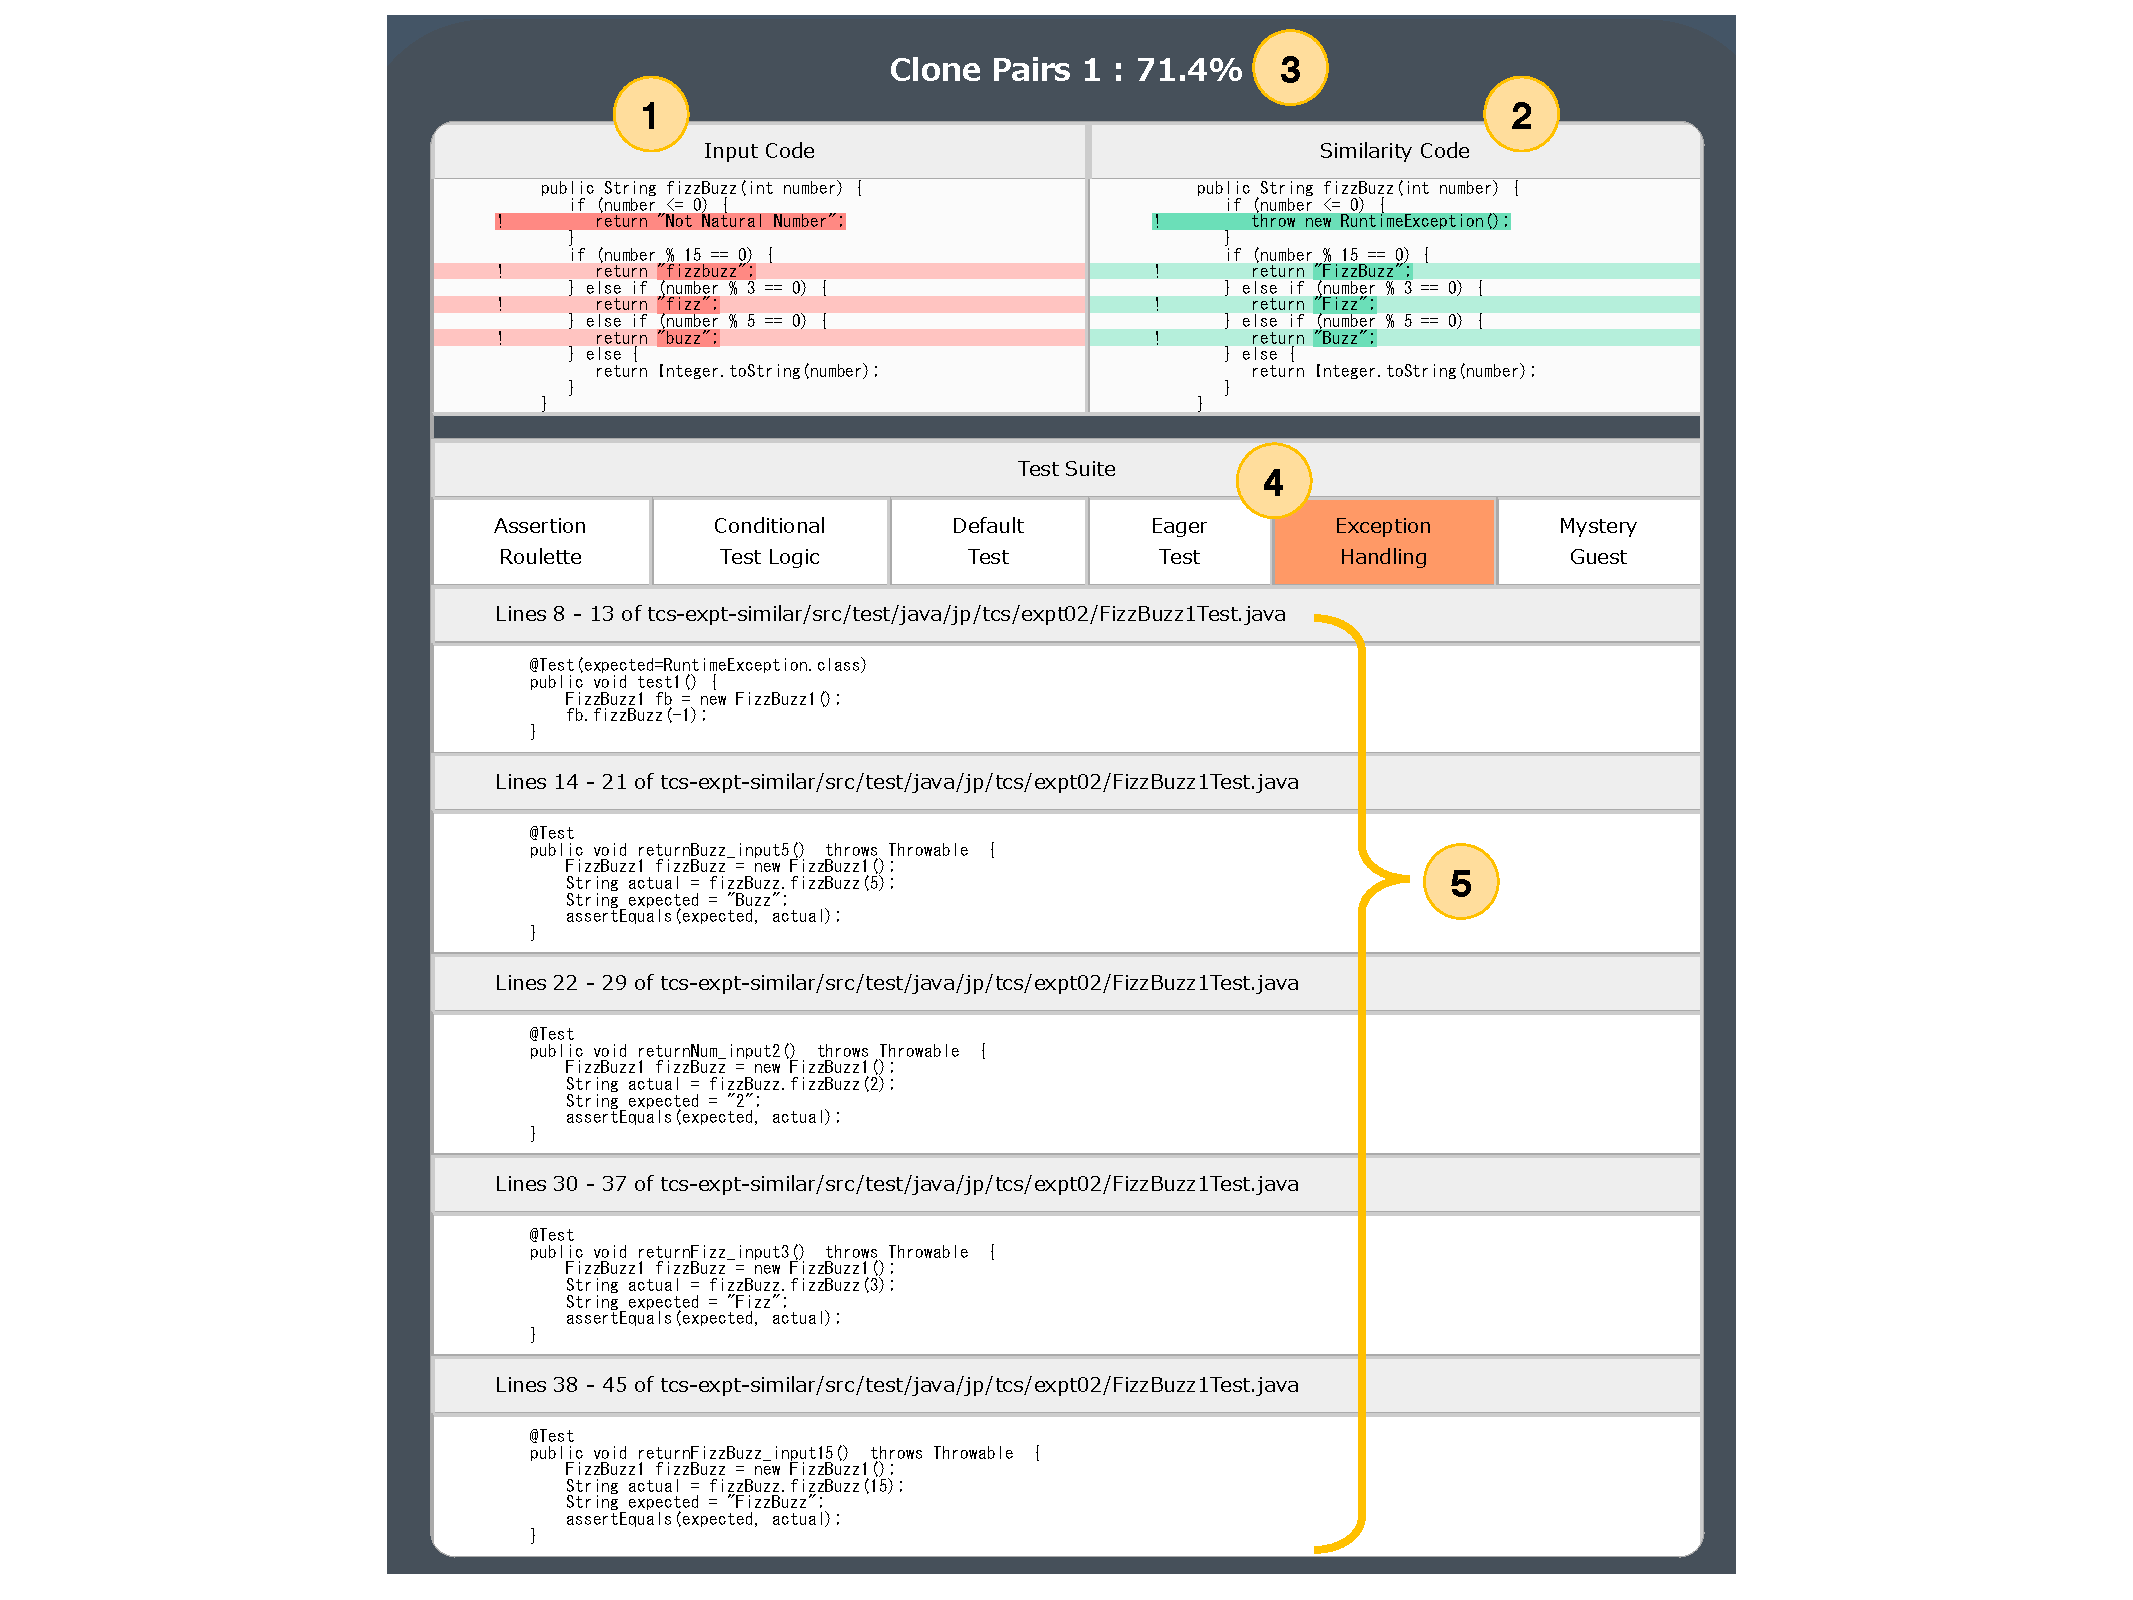
\includegraphics[width=8.7cm]{SuiteRec.pdf}}
\caption{Test suite recommended by SuiteRec.}
\label{fig}
\end{figure}

 \begin{enumerate}
\renewcommand{\labelenumi}{(\arabic{enumi})}
\item{\textbf{Input Code.}The target code entered by the developer is displayed.}
\item{\textbf{Similarity Code.}A similar code for the input code is displayed. The differences are highlighted so that you can see the difference between the input code and the similarity code.}
\item{\textbf{Degree of similarity.}The similarity between the input code and the similar code is displayed. The similarity is calculated using the Unique Percentage of Items (UPI) method used by NICAD[?].}
\item{\textbf{Test Smells.}If test smells are included in the test suite, the test smell is highlighted in orange, and the developer is presented with the presence of test smells.}
\item{\textbf{Recommend Test Suites.}The recommended test suite is displayed. A file path is also displayed to indicate from which project the test code was referenced.}
\end{enumerate}


\section{Evaluation}
In this section, we will conduct experiments with subjects to evaluate SuiteRec quantitatively and qualitatively. Subjects will be asked to create test codes for three production codes. Evaluate SuiteRec by comparing the test code with and without using SuiteRec. 

By collecting data on code coverage, time to complete experimental tasks and test code quality throughout the experiment, we aim to answer the following research questions:


\begin{itemize}
\item RQ1: \textbf{Can SuiteRec support the creation of tests with high coverage?} Coverage is an important factor as an indicator of software quality. If there is a line that is never executed in the test code, the quality of that part cannot be ensured. Can SuiteRec help increase coverage?
\item RQ2: \textbf{Can SuiteRec reduce test code creation time?} Can developers shorten test code creation time by referring to test codes recommended by SuiteRec?
\item RQ3: \textbf{Can SuiteRec support high quality test creation?} Can developers create high-quality test code by referring to the test code recommended by SuiteRec?
\item RQ4: \textbf{How do using SuiteRec influence the developers’ perception of test code creation tasks tasks? } Do developers find it easier to create test code when using SuiteRec, and are they more confident in their created test code?
\end{itemize}

\subsection{Participant Selection}
We recruited students with basic programming skills and an understanding of software testing. The experiment was conducted with 10 master students who majored in information science.According to the preliminary questionnaire, more than 90\% of the students had more than 2 years of programming experience, and more than 80\% of the subjects had more than 1 year of Java language experience. All students had basic knowledge about software testing in lectures and other lectures, and more than 80\% had experience creating unit tests.

\subsection{Object Selection}
To conduct the experiment we prepared three production codes. It is assumed that the subjects fully understand the specifications of production code in order to create test code. Therefore, we selected a typical computational problem that often uses competitive programming as production code. In addition, a specification written in natural language was prepared so that the specification of the production code could be confirmed. In order to make a difference in each task, the number of conditional branches in each task was increased to 8, 16, and 24.

Figure 4 is an example of the production code that was presented. In the post-experimental questionnaire, it was confirmed that all the subjects expressed a positive opinion about the understanding of the experimental task. Also, there was no negative answer to the question about whether there was enough experiment time. Therefore, it can be seen that the subject fully understood the given experimental task and had sufficient work time.


\begin{figure}[htbp]
\centerline{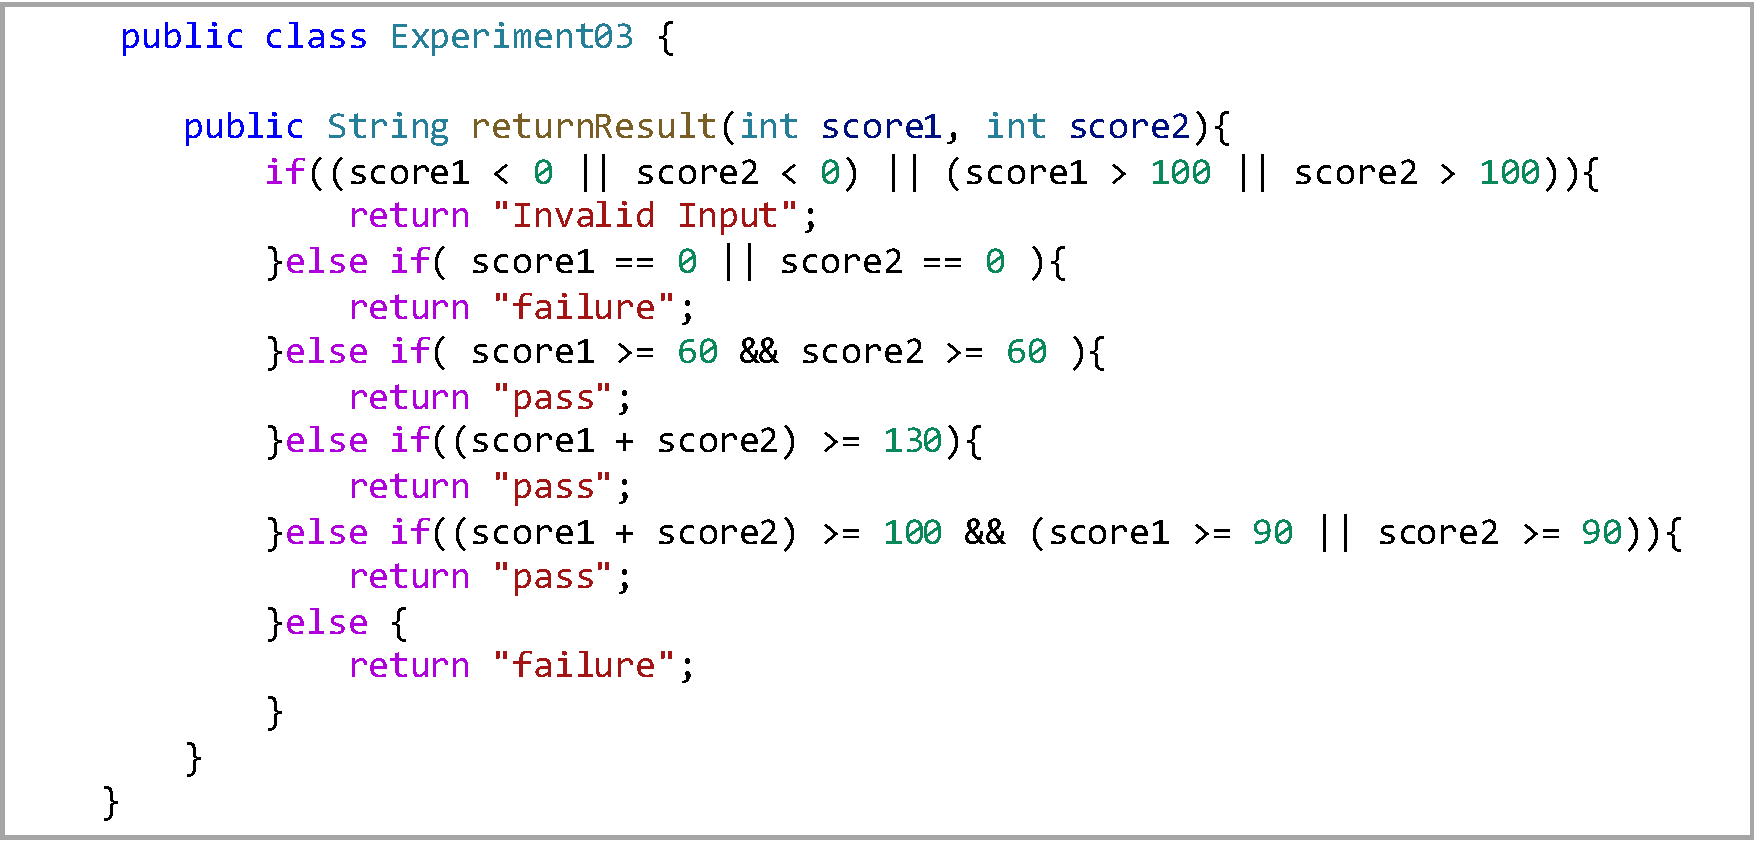
\includegraphics[width=8.5cm]{task.pdf}}
\caption{Example of a experimental task.}
\label{fig}
\end{figure}

\subsection{Experiment Procedure}
First, we conducted a 30-minute lecture and practice task on using JUnit from basic knowledge about software testing, and confirmed understanding of the test code description. And we asked them to create test codes for the three production codes for the actual experiment.

Ask the subjects to judge the end of the experimental task. Specifically, the test task was completed when the subjects were satisfied with the coverage and quality of the test code they created. The experiment time was a maximum of 25 minutes per task.

To prevent the use effect of SuiteRec from being biased by tasks, subjects were assigned to change whether or not SuiteRec was used depending on the task. In order to prevent the learning effect when SuiteRec is used, tasks are assigned so that SuiteRec is not used continuously in three tasks. The subjects were not allowed to refer to past answers.

\section{Results}
In this section we present the quantitative and qualitative evaluation results of SuiteRec by 10 subjects, as described in the previous section, for each of the research questions.

\subsection{RQ1: Can SuiteRec support the creation of tests with high coverage?}
In this experiment, we calculated two types of code coverage: statement coverage(C0) and branch coverage(C1) of test suites submitted by the subjects. To calculate the coverage, we used EclEmma[?], which is installed as a plug-in of the integrated development environment Eclipse[?]. Figures 1 and 2 show the average coverage of statement coverage and branch coverage, respectively. As a result, there is almost no difference in the coverage rate of statement coverage in all three tasks depending on whether SuiteRec is used or not, and the coverage of each task exceeds 90\%.

Regarding the branch coverage in Fig. 2, it can be seen that there is almost no difference between TASK1 and TASK2 with 8,16 branches depending on whether SuiteRec is used or not. 

However, the results of TASK3 with the largest number of branches showed that there was a difference of more than 10\% in the average coverage of the subjects.

This result suggests that the test code recommended by SuiteRec is useful for increasing the coverage rate when creating test code for production code with many branches. In fact, in the questionnaire after the experiment, there were multiple reports that the subjects were able to follow the test items that were overlooked by the recommendation code.


\begin{figure}[htbp]
\centerline{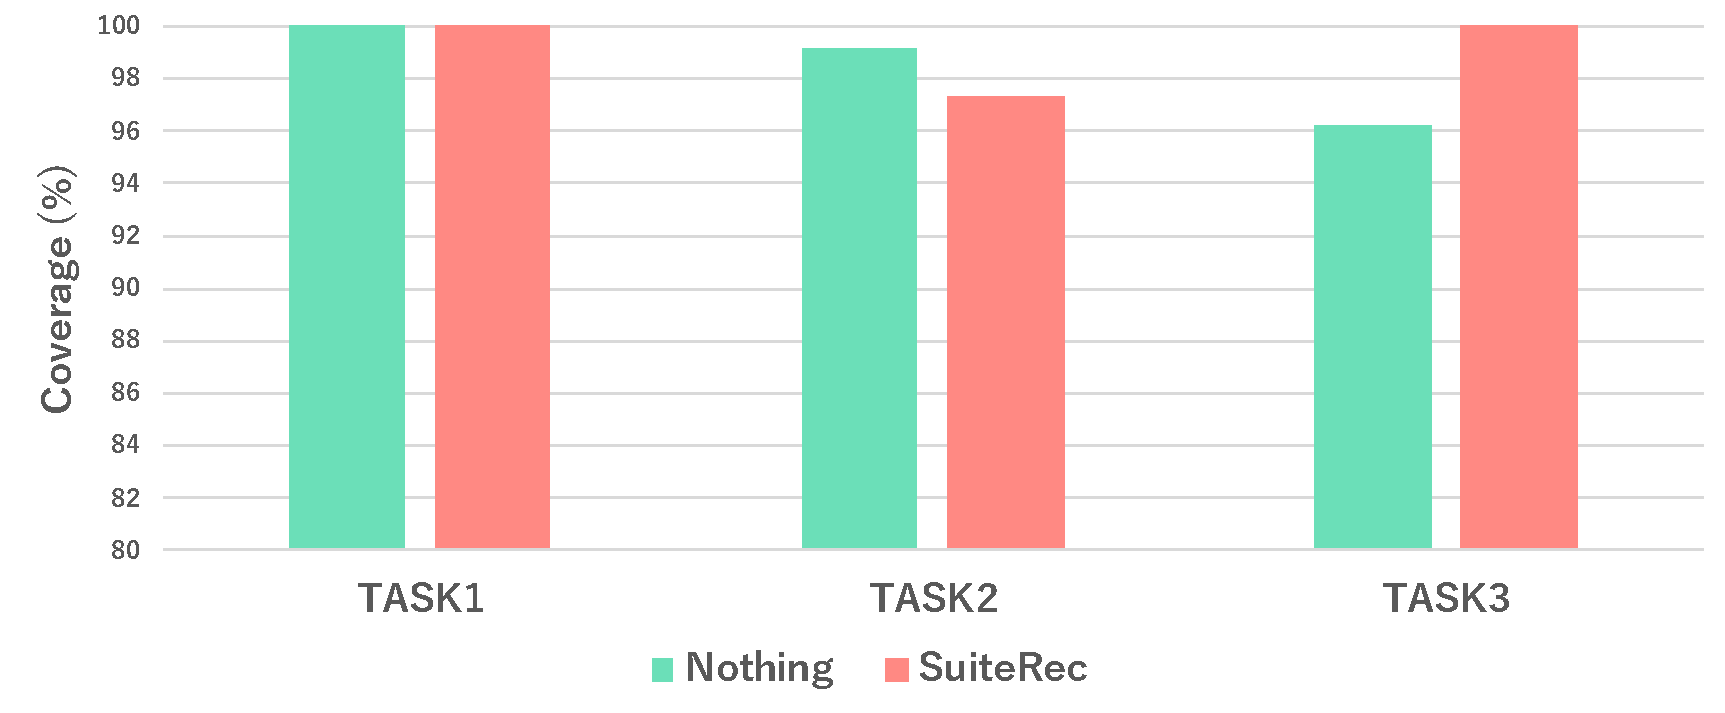
\includegraphics[width=8.5cm]{C0.pdf}}
\caption{Statement coverage (C0).}
\label{fig}
\end{figure}

\begin{figure}[htbp]
\centerline{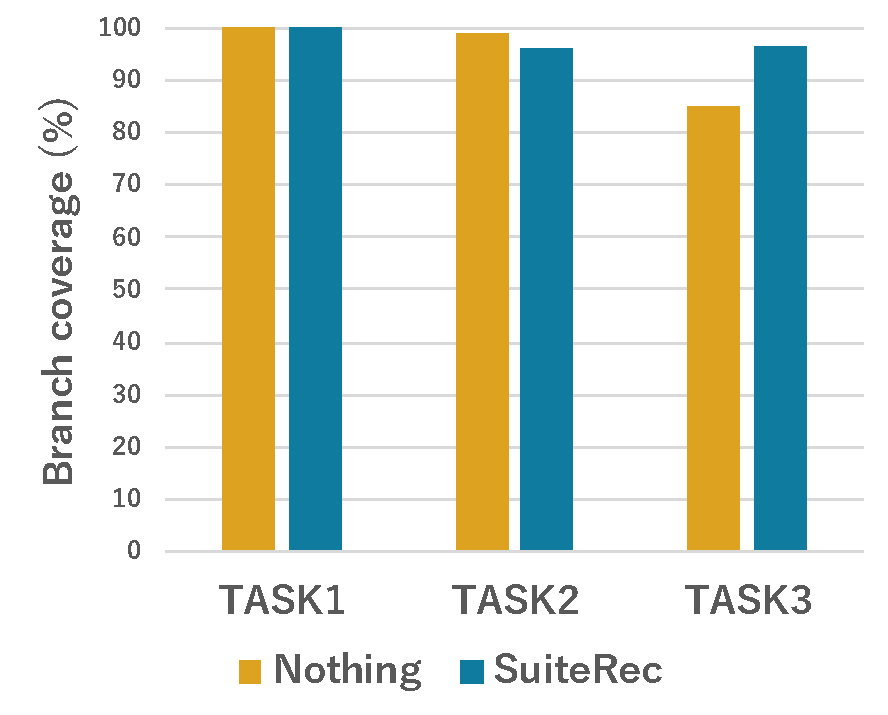
\includegraphics[width=8.5cm]{C1.pdf}}
\caption{Branch coverage (C1).}
\label{fig}
\end{figure}

\subsection{RQ2: Can SuiteRec reduce test code creation time?}
Figure 5 shows the results of comparing the time spent completing the test code creation task with and without SuiteRec. It can be seen that the test creation time is longer when SuiteRec is used for tasks 1 and 3 than when it is not. This result can take time to read and understand multiple test suites recommended by SuiteRec. Subjects will not be able to reuse the recommended test code without modification. It is necessary to rewrite the test code by looking at the difference between the input production code and the detected similar code. In addition, according to the questionnaire after the experiment, it was necessary to rewrite each time the object creation sentence was reused, and it took time.

For Task 2, it can be seen that the test creation time is shorter when SuiteRec is used. We examined the submitted test code and found that there were many test cases (items) when SuiteRec was not used, although there was no difference in coverage. This result suggests that the subjects may have wasted time creating many useless test cases.

\begin{figure}[htbp]
\centerline{\includegraphics[width=8.5cm]{duration.pdf}}
\caption{Time taken to create test code.}
\label{fig}
\end{figure}

\subsection{RQ3: Can SuiteRec support high quality test creation?}
Figure 6 shows the results of comparing the number of test smells in the submitted test code with and without SuiteRec. For all TASKs, the test code created using SuiteRec contains less test smell than if it were not used. This result suggests that the quality of the recommended test code is high, and the developer can create the test code while maintaining the quality by reusing it. Also, by presenting the test smells included in the recommended test suite, the test code may be rewritten based on it and a high quality test code may have been submitted. In the actual questionnaire responses, it was reported that the test smells presented were understood and refactored to eliminate them.

On the other hand, some subjects were aware that test smells were included, but did not know how to refactor. This is a topic for the future and needs to be improved to show how to refactor test smells.

When SuiteRec was not used, the subjects embedded more than five times the test smells compared to the case where it was used. This is probably because many subjects did not rename the default test method and wrote the Assert statement by copy and paste within one test method. In fact, it has been reported that many of these test smells are detected in existing projects [6].


\begin{figure}[htbp]
\centerline{\includegraphics[width=8.5cm]{smells.pdf}}
\caption{Number of detected test smells.}
\label{fig}
\end{figure}

\begin{figure*}[t]
 \begin{center}
  \includegraphics[width=18.5cm]{suiterec-expt.pdf}
  \caption{キャプション}
  \label{}
 \end{center}
\end{figure*}

\subsection{RQ4: How do using SuiteRec influence the developers’ perception of test code creation tasks tasks?}
Figure 7 summarizes answers to the survey questions. Overall, the subjects found the task clear (Question 1), and the allocated time sufficient (Question 2). For the remaining questions, you can see that there is a difference in opinion on the experimental task with and without SuiteRec. 

When creating test codes, subjects can easily feel test code creation using SuiteRec. However, this result contrasts with the actual task end time and length (Figure 2), and it can be seen that the task end time is slower when SuiteRec is used. The subjects read and understand the recommended multiple suggested test suites and decide whether to reuse them. In addition, the test code cannot be applied without editing, and it is necessary to understand the difference between the input code and the detected similar code and make appropriate modifications to the test code. We speculate that when using SuiteRec, subjects may spend a lot of time on this part. 

Many opinions that it is better to add a function that supports test code editing work (such as a function that automatically edits the class name and method name to the name corresponding to the input code) in the free description of the tool improvement by questionnaire I received. Further improvements in SuiteRec show the potential for reducing the completion time of experimental tasks.

When using SuiteRec, the subject is confident in the coverage of the test code created by himself (Question 5). On the other hand, 40\% of subjects reported a negative response when nothing was used. However, it is known that there is almost no difference in the coverage of the test code actually submitted (Figure 3). It is important to be confident in the coverage of the test code you create. One of the purposes of software testing is that developers are responsible for the code they write and can provide software to users without anxiety.

When the test code was created without using SuiteRec, 40\% of the subjects were not confident in the quality of the test code they wrote. It can be seen that the number of test smells in the actual submitted test code is greater when SuiteRec is not used than when it is used (Figure 4). Developers unknowingly embed test smells that make later maintenance activities difficult. The use of SuiteRec reduces the number of test mells by giving developers an awareness of the quality of the test code and brings confidence to the code they have created.

On the other hand, even when SuiteRec is used, there are negative opinions about the quality of the test code. The respondents reported that they understood Test Smells but didn't know how to refactor. This indicates the need for further improvement of SuiteRec, and we should add the function to present refactoring methods for each test smell.

\begin{comment}
\section{Related work}
\textbf{Code recommendation.}コード推薦システムは,他のプログラムのコードフラグメントを提示し再利用できるようにしたりすることで開発者を支援します.Zhang[1]らはクローンペア間で,コードを移植を行い移植前と移植後のテスト結果を比較しその情報を基にテストを再利用する手法を提案している.Mostafa[2]らは,自身のプロジェクトだけでなく他のプロジェクトを横断してクローンペアを検出しテストコード再利用することの有効性を調査した.
\end{comment}

\section{Conclusion and Future Work}
SuiteRec is a tool that recommends existing test codes that exist on OSS using a similar code detection tool for the input production code. In addition, SuiteRec presents the test smell, an indicator of poor test code implementation, to the developer, and the order of recommendation is sorted so that higher quality test suites can be recommended.

According to the evaluation of SuiteRec by 10 subjects, it may be possible to improve coverage by creating test code using SuiteRec for production code which there are many branches and it is difficult to create test items. However, it takes a lot of creation time. Using SuiteRec also allows you to create high quality test code that doesn't contain much test smells, and developers can be confident in the code they write. 

As a future task, SuiteRec needs to be improved for more practical use. Specifically, we are considering an automatic test code rewriting function. In addition, the validity of test suite priorities recommended by SuiteRec will be evaluated.


\begin{comment}

%\subsection{Maintaining the Integrity of the Specifications}

The IEEEtran class file is used to format your paper and style the text. All margins, 
column widths, line spaces, and text fonts are prescribed; please do not 
alter them. You may note peculiarities. For example, the head margin
measures proportionately more than is customary. This measurement 
and others are deliberate, using specifications that anticipate your paper 
as one part of the entire proceedings, and not as an independent document. 
Please do not revise any of the current designations.

\section{Prepare Your Paper Before Styling}
Before you begin to format your paper, first write and save the content as a 
separate text file. Complete all content and organizational editing before 
formatting. Please note sections \ref{AA}--\ref{SCM} below for more information on 
proofreading, spelling and grammar.

Keep your text and graphic files separate until after the text has been 
formatted and styled. Do not number text heads---{\LaTeX} will do that 
for you.

\subsection{Abbreviations and Acronyms}\label{AA}
Define abbreviations and acronyms the first time they are used in the text, 
even after they have been defined in the abstract. Abbreviations such as 
IEEE, SI, MKS, CGS, ac, dc, and rms do not have to be defined. Do not use 
abbreviations in the title or heads unless they are unavoidable.

\subsection{Units}
\begin{itemize}
\item Use either SI (MKS) or CGS as primary units. (SI units are encouraged.) English units may be used as secondary units (in parentheses). An exception would be the use of English units as identifiers in trade, such as ``3.5-inch disk drive''.
\item Avoid combining SI and CGS units, such as current in amperes and magnetic field in oersteds. This often leads to confusion because equations do not balance dimensionally. If you must use mixed units, clearly state the units for each quantity that you use in an equation.
\item Do not mix complete spellings and abbreviations of units: ``Wb/m\textsuperscript{2}'' or ``webers per square meter'', not ``webers/m\textsuperscript{2}''. Spell out units when they appear in text: ``. . . a few henries'', not ``. . . a few H''.
\item Use a zero before decimal points: ``0.25'', not ``.25''. Use ``cm\textsuperscript{3}'', not ``cc''.)
\end{itemize}

\subsection{Equations}
Number equations consecutively. To make your 
equations more compact, you may use the solidus (~/~), the exp function, or 
appropriate exponents. Italicize Roman symbols for quantities and variables, 
but not Greek symbols. Use a long dash rather than a hyphen for a minus 
sign. Punctuate equations with commas or periods when they are part of a 
sentence, as in:
\begin{equation}
a+b=\gamma\label{eq}
\end{equation}

Be sure that the 
symbols in your equation have been defined before or immediately following 
the equation. Use ``\eqref{eq}'', not ``Eq.~\eqref{eq}'' or ``equation \eqref{eq}'', except at 
the beginning of a sentence: ``Equation \eqref{eq} is . . .''

\subsection{\LaTeX-Specific Advice}

Please use ``soft'' (e.g., \verb|\eqref{Eq}|) cross references instead
of ``hard'' references (e.g., \verb|(1)|). That will make it possible
to combine sections, add equations, or change the order of figures or
citations without having to go through the file line by line.

Please don't use the \verb|{eqnarray}| equation environment. Use
\verb|{align}| or \verb|{IEEEeqnarray}| instead. The \verb|{eqnarray}|
environment leaves unsightly spaces around relation symbols.

Please note that the \verb|{subequations}| environment in {\LaTeX}
will increment the main equation counter even when there are no
equation numbers displayed. If you forget that, you might write an
article in which the equation numbers skip from (17) to (20), causing
the copy editors to wonder if you've discovered a new method of
counting.

{\BibTeX} does not work by magic. It doesn't get the bibliographic
data from thin air but from .bib files. If you use {\BibTeX} to produce a
bibliography you must send the .bib files. 

{\LaTeX} can't read your mind. If you assign the same label to a
subsubsection and a table, you might find that Table I has been cross
referenced as Table IV-B3. 

{\LaTeX} does not have precognitive abilities. If you put a
\verb|\label| command before the command that updates the counter it's
supposed to be using, the label will pick up the last counter to be
cross referenced instead. In particular, a \verb|\label| command
should not go before the caption of a figure or a table.

Do not use \verb|\nonumber| inside the \verb|{array}| environment. It
will not stop equation numbers inside \verb|{array}| (there won't be
any anyway) and it might stop a wanted equation number in the
surrounding equation.

\subsection{Some Common Mistakes}\label{SCM}
\begin{itemize}
\item The word ``data'' is plural, not singular.
\item The subscript for the permeability of vacuum $\mu_{0}$, and other common scientific constants, is zero with subscript formatting, not a lowercase letter ``o''.
\item In American English, commas, semicolons, periods, question and exclamation marks are located within quotation marks only when a complete thought or name is cited, such as a title or full quotation. When quotation marks are used, instead of a bold or italic typeface, to highlight a word or phrase, punctuation should appear outside of the quotation marks. A parenthetical phrase or statement at the end of a sentence is punctuated outside of the closing parenthesis (like this). (A parenthetical sentence is punctuated within the parentheses.)
\item A graph within a graph is an ``inset'', not an ``insert''. The word alternatively is preferred to the word ``alternately'' (unless you really mean something that alternates).
\item Do not use the word ``essentially'' to mean ``approximately'' or ``effectively''.
\item In your paper title, if the words ``that uses'' can accurately replace the word ``using'', capitalize the ``u''; if not, keep using lower-cased.
\item Be aware of the different meanings of the homophones ``affect'' and ``effect'', ``complement'' and ``compliment'', ``discreet'' and ``discrete'', ``principal'' and ``principle''.
\item Do not confuse ``imply'' and ``infer''.
\item The prefix ``non'' is not a word; it should be joined to the word it modifies, usually without a hyphen.
\item There is no period after the ``et'' in the Latin abbreviation ``et al.''.
\item The abbreviation ``i.e.'' means ``that is'', and the abbreviation ``e.g.'' means ``for example''.
\end{itemize}
An excellent style manual for science writers is \cite{b7}.

\subsection{Authors and Affiliations}
\textbf{The class file is designed for, but not limited to, six authors.} A 
minimum of one author is required for all conference articles. Author names 
should be listed starting from left to right and then moving down to the 
next line. This is the author sequence that will be used in future citations 
and by indexing services. Names should not be listed in columns nor group by 
affiliation. Please keep your affiliations as succinct as possible (for 
example, do not differentiate among departments of the same organization).

\subsection{Identify the Headings}
Headings, or heads, are organizational devices that guide the reader through 
your paper. There are two types: component heads and text heads.

Component heads identify the different components of your paper and are not 
topically subordinate to each other. Examples include Acknowledgments and 
References and, for these, the correct style to use is ``Heading 5''. Use 
``figure caption'' for your Figure captions, and ``table head'' for your 
table title. Run-in heads, such as ``Abstract'', will require you to apply a 
style (in this case, italic) in addition to the style provided by the drop 
down menu to differentiate the head from the text.

Text heads organize the topics on a relational, hierarchical basis. For 
example, the paper title is the primary text head because all subsequent 
material relates and elaborates on this one topic. If there are two or more 
sub-topics, the next level head (uppercase Roman numerals) should be used 
and, conversely, if there are not at least two sub-topics, then no subheads 
should be introduced.

\subsection{Figures and Tables}
\paragraph{Positioning Figures and Tables} Place figures and tables at the top and 
bottom of columns. Avoid placing them in the middle of columns. Large 
figures and tables may span across both columns. Figure captions should be 
below the figures; table heads should appear above the tables. Insert 
figures and tables after they are cited in the text. Use the abbreviation 
``Fig.~\ref{fig}'', even at the beginning of a sentence.

\begin{table}[htbp]
\caption{Table Type Styles}
\begin{center}
\begin{tabular}{|c|c|c|c|}
\hline
\textbf{Table}&\multicolumn{3}{|c|}{\textbf{Table Column Head}} \\
\cline{2-4} 
\textbf{Head} & \textbf{\textit{Table column subhead}}& \textbf{\textit{Subhead}}& \textbf{\textit{Subhead}} \\
\hline
copy& More table copy$^{\mathrm{a}}$& &  \\
\hline
\multicolumn{4}{l}{$^{\mathrm{a}}$Sample of a Table footnote.}
\end{tabular}
\label{tab1}
\end{center}
\end{table}

\begin{figure}[htbp]
\centerline{\includegraphics{fig1.pdf}}
\caption{Example of a figure caption.}
\label{fig}
\end{figure}

Figure Labels: Use 8 point Times New Roman for Figure labels. Use words 
rather than symbols or abbreviations when writing Figure axis labels to 
avoid confusing the reader. As an example, write the quantity 
``Magnetization'', or ``Magnetization, M'', not just ``M''. If including 
units in the label, present them within parentheses. Do not label axes only 
with units. In the example, write ``Magnetization (A/m)'' or ``Magnetization 
\{A[m(1)]\}'', not just ``A/m''. Do not label axes with a ratio of 
quantities and units. For example, write ``Temperature (K)'', not 
``Temperature/K''.

\section*{Acknowledgment}

The preferred spelling of the word ``acknowledgment'' in America is without 
an ``e'' after the ``g''. Avoid the stilted expression ``one of us (R. B. 
G.) thanks $\ldots$''. Instead, try ``R. B. G. thanks$\ldots$''. Put sponsor 
acknowledgments in the unnumbered footnote on the first page.

\section*{References}

Please number citations consecutively within brackets \cite{b1}. The 
sentence punctuation follows the bracket \cite{b2}. Refer simply to the reference 
number, as in \cite{b3}---do not use ``Ref. \cite{b3}'' or ``reference \cite{b3}'' except at 
the beginning of a sentence: ``Reference \cite{b3} was the first $\ldots$''

Number footnotes separately in superscripts. Place the actual footnote at 
the bottom of the column in which it was cited. Do not put footnotes in the 
abstract or reference list. Use letters for table footnotes.

Unless there are six authors or more give all authors' names; do not use 
``et al.''. Papers that have not been published, even if they have been 
submitted for publication, should be cited as ``unpublished'' \cite{b4}. Papers 
that have been accepted for publication should be cited as ``in press'' \cite{b5}. 
Capitalize only the first word in a paper title, except for proper nouns and 
element symbols.

For papers published in translation journals, please give the English 
citation first, followed by the original foreign-language citation \cite{b6}.

\end{comment}

\begin{thebibliography}{00}
\bibitem{b1} S. Shamshiri, J. M. Rojas, J. P. Galeotti, ``How Do Automatically Generated Unit Tests Influence Software Maintenance?," In {\it Proceedings of the International Conference on Software Testing, Verification and Validation (ICST)}, pp.239--249, 2018. 

\bibitem{b2} C. K. Roy and J. R. Cordy, ``NICAD: Accurate Detection of Near-Miss Intentional Clones Using Flexible Pretty-Printing and Code Normalization," In {\it Proceedings of the International Conference on Program Comprehension (ICPC)}, pp.172--181, 2008.

\bibitem{b3} G. Fraser and A. Arcuri, ``EvoSuite: automatic test suite generation for object-oriented software," in  {\it Proceedings of the Symposium on the Foundations of Software Engineering (FSE)}, pp. 416--419, 2011.

\bibitem{b4} N. Koochakzadeh and V. Garousi, ``Tecrevis: a tool for test coverage and test redundancyvisualization," Testing–Practice and Research Techniques, 2010.

\bibitem{b5} M.Greiler, A.Zaidman, A.v.Deursen, and M.-A.Storey, ``Strategies for avoiding text fixture smells during software evolution," In {\it Proceedings of the 10th Working Conference on Mining Software Repositories (MSR)}, pp. 387--396, 2013.

\bibitem{b6} G. Meszaros. xUnit Test Patterns: Refactoring Test Code. Addison Wesley, 2007.

\bibitem{b7} A. van Deursen, L. Moonen, A. Bergh, G. Kok. Refactoring test code. In {\it Proceedings of the 2nd International Conference on Extreme Programming and Flexible Processes in Software Engineering (XP)}, pp. 92--95, 2001.

\bibitem{b8} D. Spadini, F. Palomba, A. Zaiaman, M. Bruntink, A.Bacchelli, ``On The Relation of Test Smells to Software Code Quality," In {\it Proceedings of the International Conference on Software Maintenance and Evolution (ICSME)}, pp. 1--12, 2018. 

\bibitem{b9} A. Peruma, K. Almalki, C. D. Newman, M. W. Mkaouer, A. Ouni, F. Palomba, ``On the distribution of test smells in open source Android applications: an exploratory study," In {\it Proceedings of the International Conference on Computer Science and Software Engineering (CASCON)}, pp. 193--202, 2019.

\bibitem{b10} S. U. T. Smells. http://testsmells.github.io/, 2018.

\bibitem{b11} https://www.eclemma.org/

\bibitem{b12} P. Machado and A. Sampaio, ``Automatic Test-Case Generation," Testing Techniques in Software Eng., vol. 6153, pp. 59--103, 2010. 

\bibitem{b13} S. Panichella, A. Panichella, M. Beller, A. Zaidman, and H. C. Gall, ``The impact of test case summaries on bug fixing performance: An empirical investigation," In {\it Proceedings of the International Conference on Software Engineering (ICSE)}, pp. 547--558, 2016.

\bibitem{b14} E. Daka, J. Campos, G. Fraser, J. Dorn, and W. Weimer, ``Modeling readability to improve unit tests," In {\it Proceedings of the Joint Meeting on Foundations of Software Engineering (ESEC/FSE)}, pp. 107--118, 2015.

\bibitem{b15} F. Palomba, A. Panichella, A. Zaidman, R. Oliveto, and A. De Lucia, ``Automatic test case generation: what if test code quality matters?," In {\it Proceedings of the International Symposium on Software Testing and Analysis (ISSTA)}, pp. 130--141, 2016.

\begin{comment}
\bibitem{b1} G. Eason, B. Noble, and I. N. Sneddon, ``On certain integrals of Lipschitz-Hankel type involving products of Bessel functions,'' Phil. Trans. Roy. Soc. London, vol. A247, pp. 529--551, April 1955.
\bibitem{b2} J. Clerk Maxwell, A Treatise on Electricity and Magnetism, 3rd ed., vol. 2. Oxford: Clarendon, 1892, pp.68--73.
\bibitem{b3} I. S. Jacobs and C. P. Bean, ``Fine particles, thin films and exchange anisotropy,'' in Magnetism, vol. III, G. T. Rado and H. Suhl, Eds. New York: Academic, 1963, pp. 271--350.
\bibitem{b4} K. Elissa, ``Title of paper if known,'' unpublished.
\bibitem{b5} R. Nicole, ``Title of paper with only first word capitalized,'' J. Name Stand. Abbrev., in press.
\bibitem{b6} Y. Yorozu, M. Hirano, K. Oka, and Y. Tagawa, ``Electron spectroscopy studies on magneto-optical media and plastic substrate interface,'' IEEE Transl. J. Magn. Japan, vol. 2, pp. 740--741, August 1987 [Digests 9th Annual Conf. Magnetics Japan, p. 301, 1982].
\bibitem{b7} M. Young, The Technical Writer's Handbook. Mill Valley, CA: University Science, 1989.
\end{comment}
\end{thebibliography}


\begin{comment}
\vspace{12pt}
\color{red}
IEEE conference templates contain guidance text for composing and formatting conference papers. Please ensure that all template text is removed from your conference paper prior to submission to the conference. Failure to remove the template text from your paper may result in your paper not being published.
\end{comment}
\end{document}
